%% Method. POSD is the centrepiece; augmentation supplies its views. OPERA = the two. OPERA++ = plus harsh-pool
%% mining, reported as a variant. Mining over the training mixture is a control, never an arm.
%% Included by sigconf.tex. Do not add a preamble here.

\section{Privileged Observation Self-Distillation}
\label{sec:method}

\begin{figure}[t]
\centering
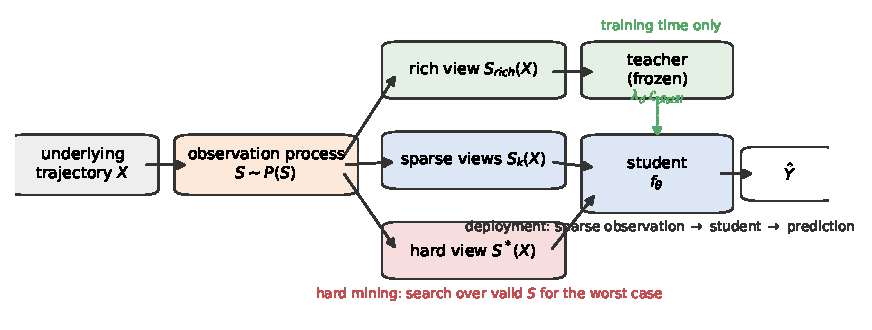
\includegraphics[width=\linewidth]{figures/fig1_framework.pdf}
\caption{The student is restricted to a sparse observation of a trajectory; the teacher receives a richer
observation of the \emph{same history}, over the same prediction times and with the same supervision, and its
task output becomes an additional target for the student (dashed). Observation-process augmentation supplies the
student's views. OPERA is these two mechanisms; OPERA++ additionally replaces some views with the hardest
candidate from a pool harsher than the training mixture. At deployment only the student and one sparse
observation remain.}
\label{fig:framework}
\end{figure}

Everything in this section acts on $\Sobs$ rather than on the encoder: the architecture, its parameter count and
its inference path are untouched (Figure~\ref{fig:framework}). Two configurations are reported, and the
distinction matters because one mechanism turns out to be conditional on a hyper-parameter rather than
universally useful:
\begin{itemize}
\item \textbf{OPERA} $=$ privileged observation self-distillation $+$ observation-process augmentation. This is
the method: two mechanisms, no candidate pool to choose.
\item \textbf{OPERA++} $=$ OPERA $+$ hard observation-process mining from a pool strictly harsher than the
training mixture. It buys worst-case robustness for $K$ extra forward passes per step and one more
hyper-parameter.
\end{itemize}
Mining over the training mixture itself is neither configuration. It is the control that establishes why pool
severity matters, and we report it as an ablation (Section~\ref{sec:mining-results}). We introduce distillation
first, as the mechanism we regard as the contribution, then the augmentation that feeds it, then the objective
that defines OPERA, and finally the mining variant.

\subsection{Rich and sparse observations of one history}
\label{sec:distill}
At deployment a model receives whatever its observation process supplies. During training the same history can be
re-observed at will, and in particular it can be observed \emph{more richly} than deployment permits. Write
\begin{equation}
\Oobs_s=\Sobs_s(X),\qquad \Oobs_r=\Sobs_r(X),
\label{eq:richsparse}
\end{equation}
where $\Sobs_s$ is a deployment-constrained observation process and $\Sobs_r$ is at least as dense as $\Sobs_s$ on
the same trajectory; in our experiments $\Sobs_r$ is the untouched record. Because $\Oobs_r$ exists only at
training time it is privileged information in the sense of \cite{vapnik2015lupi}, and distillation
\cite{hinton2015distilling,lopezpaz2016unifying} is the natural way to route it into the student.

\subsection{The distillation objective}
A teacher $f_{\theta_T}$ is trained on rich observations and then frozen. The student $f_\theta$ is trained on
sparse observations of the same histories and, in addition to the task loss, is asked to reproduce the teacher's
task-level output:
\begin{equation}
\hat Y_T=f_{\theta_T}(\Oobs_r),\qquad \hat Y_S=f_\theta(\Oobs_s),
\label{eq:studteach}
\end{equation}
\begin{equation}
\mathcal{L}_{\mathrm{distill}}=D\big(\hat Y_S,\ \mathrm{sg}[\hat Y_T]\big)
=\big\|\hat Y_S-\mathrm{sg}[\hat Y_T]\big\|^{2}_{\Omega},
\label{eq:distill}
\end{equation}
where $\mathrm{sg}[\cdot]$ is the stop-gradient and $\Omega$ restricts the norm to entries that carry supervision,
so the student is never asked to imitate the teacher where no target exists. For probabilistic outputs $D$ may
instead be a KL divergence. We also implement an exponential-moving-average teacher,
$\theta_T\leftarrow\alpha_T\theta_T+(1-\alpha_T)\theta$, and treat frozen-versus-EMA as an empirical choice; the
reported runs use a frozen teacher.

The value of this term is not that the teacher is a better model. Teacher and student share capacity, family and
objective, and the teacher is ahead only because less of the trajectory was discarded before it saw it. Its output
describes what is predictable from that trajectory under a smaller observation loss, and the student is pushed
toward that value from a view in which part of the same structure has been removed. Stated precisely, the teacher
exposes the student to prediction-relevant information that is present in the underlying history but partially
obscured by the deployment observation process. It does not tell the student which observations will be available:
that is fixed by the deployment process and is not something the student can act on.

\paragraph{Why the teacher has something to offer.}
Section~\ref{sec:family} noted that a variable is predicted from the whole observation, not from its own channel,
so removing one channel degrades the others. The converse is what makes the rich view informative: an observation
that retains channels the student's view lost supports a prediction the student cannot reconstruct from what it
holds. The teacher's output is a summary of that, at exactly the granularity the task is scored on.

\paragraph{Why this is self-distillation.}
The asymmetry between the two networks lies entirely in the observation. The teacher is not a separately designed
expert, a larger network, or a model solving a different task; it is the same predictive model family evaluated on
a richer view of the same sample. Teacher--student distillation is not new and we do not claim it is. What is
specific here is the \emph{source and structure of the privileged signal}: it is produced by choosing a different
observation process for a history the student already holds, which requires no extra annotation, no extra sensor
and no extra data. In our experiments it also requires no extra training run, because the teacher is the
unmodified baseline for the same setting, backbone and seed.

\paragraph{The anti-leakage invariant.}
Teacher and student must differ \emph{only} in the observation of the history. Both are evaluated over the same
history window, the same prediction times and the same supervision, so the teacher never sees a future value or a
label that the student is denied. Without this restriction the term would degenerate into label leakage and any
apparent gain would be uninterpretable. We enforce it with an assertion over every batch key that carries
supervision, for both forecasting and classification, and test it directly.

\paragraph{At inference.}
The student consumes one sparse observation and emits a prediction. The teacher, the rich view and the extra
forward pass are training-time constructs; the student never receives a rich observation at test time.

\subsection{Observation-process augmentation}
\label{sec:aug}
Privileged distillation needs the student to be trained on sparse views, and the views it trains on determine what
it has to recover. The supporting mechanism supplies them by treating the observation process as nuisance
variation to randomise over: for each training trajectory we draw $V$ processes from a mixture $P_{\mathrm{mix}}$
and train on every resulting view,
\begin{equation}
\Oobs_v=\Sobs_v(X),\quad \Sobs_v\sim P_{\mathrm{mix}},\qquad
\mathcal{L}_{\mathrm{task}}=\frac1V\sum_{v=1}^{V}\ell\big(f_\theta(\Oobs_v),\,Y\big),
\label{eq:aug}
\end{equation}
with $\ell$ the masked mean squared error for forecasting and cross-entropy for classification. The targets $Y$
are shared across views and never modified: every view is a different recording of the same episode. The mixture
spans all three dimensions of Section~\ref{sec:family}, since exposure to one of them does not confer robustness
to the others.

We impose no representation-level requirement. The property we want is that $f_\theta(\Sobs_1(X))$ and
$f_\theta(\Sobs_2(X))$ both remain useful for the task, which is weaker than requiring the latent codes
$z(\Sobs_1(X))$ and $z(\Sobs_2(X))$ to agree. The weaker property is the safer one: a representation-matching
penalty admits the degenerate solution of collapsing all observations of all trajectories together, and preventing
that needs anti-collapse machinery unrelated to the shift under study. A representation-matching variant exists in
our implementation and is reported only as an ablation.

\subsection{The objective, and what OPERA is}
OPERA adds one term to the task loss,
\begin{equation}
\fbox{$\displaystyle\ \mathcal{L}=\mathcal{L}_{\mathrm{task}}+\lambda_{d}\,\mathcal{L}_{\mathrm{distill}}\ $}
\label{eq:objective}
\end{equation}
with $\mathcal{L}_{\mathrm{task}}$ from Eq.~\ref{eq:aug} over $V$ augmented views and
$\mathcal{L}_{\mathrm{distill}}$ from Eq.~\ref{eq:distill} against the frozen rich-view teacher. No other loss is
introduced, and in particular no representation-consistency term. Setting $\lambda_d=0$ and $V=1$ recovers
ordinary training. We use $\lambda_d=1$, $V=2$ and a frozen teacher throughout. Algorithm~\ref{alg:opera} is a
single update: one loss, one backward pass, one optimiser step, and the only staging is that the teacher is
trained beforehand --- which in our setup costs nothing extra, since it is the baseline run for that cell.

\begin{algorithm}[t]
\caption{One OPERA training step (OPERA++ adds the bracketed branch)}
\label{alg:opera}
\begin{algorithmic}[1]
\Require batch $(X,Y)$ with observation $(t,m)$; mixture $P_{\mathrm{mix}}$; frozen teacher $f_{\theta_T}$;
\emph{for OPERA++:} epoch $e$, pool $\mathcal{P}$, constraints $\mathcal{C}$, ratio $\alpha$
\State $\{\Sobs_v\}_{v=1}^{V}\sim P_{\mathrm{mix}}$
\If{OPERA++ \textbf{and} $e\ge e_{\mathrm{warm}}$}
  \State draw $K$ candidates from $\mathcal{P}$; keep those satisfying $\mathcal{C}$
  \State score survivors with $f_\theta$ under \texttt{no\_grad}; replace $\lceil\alpha V\rceil$ views with the hardest
\EndIf
\State $\hat{Y}_T \gets \mathrm{sg}\big[f_{\theta_T}(\Sobs_{r}(X))\big]$ \Comment{same history, richer view}
\State $\mathcal{L}\gets\frac1V\sum_v \ell(f_\theta(\Sobs_v(X)),Y) + \lambda_d\sum_v \mathcal{L}_{\mathrm{distill}}$
\State one optimiser step on $\mathcal{L}$
\end{algorithmic}
\end{algorithm}

\subsection{OPERA++: hard observation-process mining}
\label{sec:mining}
Random exposure spends most of its budget on observation processes the model already handles. The variant searches
instead for the admissible process the \emph{current} model handles worst,
\begin{equation}
\Sobs^{*}=\arg\max_{\Sobs\in\mathcal{A}}\ \ell\big(f_\theta(\Sobs(X)),Y\big),
\qquad \mathcal{A}=\{\Sobs:\ \Sobs\ \mathrm{satisfies}\ \mathcal{C}\},
\label{eq:mining}
\end{equation}
with $\mathcal{C}$ from Eq.~\ref{eq:constraints}. We do not differentiate through mask generation. We approximate
the maximisation by scoring a finite candidate pool: $K$ candidates are drawn from a pool $\mathcal{P}$, filtered
through $\mathcal{C}$, scored under \texttt{no\_grad}, and the hardest survivors retained. Only selected views
enter the backward pass, so mining costs $K$ extra forward passes and no extra gradient memory. We call this hard
observation-process mining, or approximate worst-case observation-process selection, rather than adversarial
training: the maximisation runs over a discrete pool of physically valid recordings rather than a norm ball, and it
is neither exact nor differentiable.

Training only on hard views destabilises optimisation and biases the student away from the deployment regime, so
we mix,
\begin{equation}
P(\Sobs)=(1-\alpha)\,P_{\mathrm{mix}}+\alpha\,P_{\mathrm{hard}},
\label{eq:alpha}
\end{equation}
and hold $\alpha=0$ during a warm-up period; we use $K=4$ and $\alpha=0.5$ after five epochs. The consequential
choice is $\mathcal{P}$. If $\mathcal{P}=P_{\mathrm{mix}}$ then the hardest of $K$ draws is close in severity to a
single draw and the mechanism reduces to augmentation at $K$ times the cost. OPERA++ is therefore \emph{defined}
by a pool strictly harsher than $P_{\mathrm{mix}}$, and the matched-pool setting is reported only as the control
that establishes the distinction (Section~\ref{sec:mining-results}).
